% ============================================================================
% ESQUELETO DEL INFORME - EXPOSICION MDD (UML A CODIGO)
% Asignatura: Ingenieria de Requisitos (ISR-401)
% Compilacion recomendada en TeXstudio/MiKTeX:
%   1. PdfLaTeX
%   2. BibTeX
%   3. PdfLaTeX
%   4. PdfLaTeX
% ============================================================================

\documentclass[12pt,a4paper]{article}

% ---------------------------------------------------------------------------
% CODIFICACION, IDIOMA Y TIPOGRAFIA
% ---------------------------------------------------------------------------
\usepackage[utf8]{inputenc}
\usepackage[T1]{fontenc}
\usepackage[provide=*,spanish]{babel}
\usepackage{lmodern}
\usepackage{microtype}

% ---------------------------------------------------------------------------
% CONFIGURACION DE PAGINA
% ---------------------------------------------------------------------------
\usepackage[a4paper,top=2.5cm,bottom=2.5cm,left=2.8cm,right=2.5cm]{geometry}
\usepackage{setspace}
\setstretch{1.15}
\setlength{\parindent}{0pt}
\setlength{\parskip}{0.25em}

% ---------------------------------------------------------------------------
% COLORES INSTITUCIONALES Y TITULOS
% ---------------------------------------------------------------------------
\usepackage[dvipsnames,table]{xcolor}
\definecolor{VerdeUTEQ}{HTML}{125B38}
\definecolor{AzulUTEQ}{HTML}{005A8D}
\definecolor{GrisTexto}{HTML}{333333}

\usepackage{titlesec}
\titleformat{\section}
  {\normalfont\Large\bfseries\color{VerdeUTEQ}}
  {\thesection.}{0.6em}{}
\titleformat{\subsection}
  {\normalfont\large\bfseries\color{AzulUTEQ}}
  {\thesubsection.}{0.6em}{}
\titleformat{\subsubsection}
  {\normalfont\normalsize\bfseries\color{GrisTexto}}
  {\thesubsubsection.}{0.6em}{}
\titlespacing*{\section}{0pt}{1.2em}{0.7em}
\titlespacing*{\subsection}{0pt}{1em}{0.45em}
\titlespacing*{\subsubsection}{0pt}{0.8em}{0.35em}

% ---------------------------------------------------------------------------
% FIGURAS, TABLAS Y CODIGO
% ---------------------------------------------------------------------------
\usepackage{graphicx}
\graphicspath{{figuras/}}
\usepackage{float}
\usepackage{caption}
\usepackage{booktabs}
\usepackage{array}
\usepackage{tabularx}
\usepackage{longtable}
\usepackage{listings}
\usepackage{enumitem}

\captionsetup{font=small,labelfont=bf}

\lstdefinestyle{codigoCSharp}{
  language=[Sharp]C,
  basicstyle=\ttfamily\small,
  keywordstyle=\color{AzulUTEQ}\bfseries,
  commentstyle=\color{VerdeUTEQ},
  stringstyle=\color{BrickRed},
  numbers=left,
  numberstyle=\tiny\color{gray},
  frame=single,
  breaklines=true,
  showstringspaces=false
}

% ---------------------------------------------------------------------------
% ENCABEZADO Y PIE DE PAGINA
% ---------------------------------------------------------------------------
\usepackage{fancyhdr}
\pagestyle{fancy}
\fancyhf{}
\fancyhead[L]{\small Ingeniería de Requisitos (ISR-401)}
\fancyhead[R]{\small MDD: UML a código}
\fancyfoot[C]{\thepage}
\renewcommand{\headrulewidth}{0.4pt}
\renewcommand{\footrulewidth}{0pt}
\setlength{\headheight}{15pt}

% ---------------------------------------------------------------------------
% HIPERVINCULOS E INDICE
% ---------------------------------------------------------------------------
\usepackage{xurl}
\usepackage{hyperref}
\hypersetup{
  colorlinks=true,
  linkcolor=VerdeUTEQ,
  citecolor=AzulUTEQ,
  urlcolor=AzulUTEQ,
  pdftitle={Exposición MDD con StarUML: UML a código},
  pdfauthor={Equipo de trabajo},
  pdfsubject={Ingeniería de Requisitos}
}

\setcounter{tocdepth}{3}
\setcounter{secnumdepth}{3}

% ---------------------------------------------------------------------------
% DATOS EDITABLES DE LA CARATULA
% ---------------------------------------------------------------------------
\newcommand{\Universidad}{UNIVERSIDAD TÉCNICA ESTATAL DE QUEVEDO}
\newcommand{\Facultad}{Facultad de Ciencias de la Computación y Diseño Digital}
\newcommand{\Carrera}{Carrera de Ingeniería en Software}
\newcommand{\Asignatura}{Ingeniería de Requisitos (ISR-401)}
\newcommand{\Docente}{Ing. Gleiston Guerrero Ulloa, PhD.}
\newcommand{\Periodo}{2026--2027 PPA}
\newcommand{\Paralelo}{4.º Software ``A''}
\newcommand{\NombrePFC}{Sistema de Gestión para un Gimnasio}
\newcommand{\Subsistema}{Gestión de clientes, membresías y pagos}
\newcommand{\URLRepositorio}{https://github.com/Erick-Mera/GA_Exposicion_Segundo_Corte}
\newcommand{\LugarFecha}{Quevedo -- Ecuador\\2026}

% Comando auxiliar: agrega secciones sin numerar al indice.
\newcommand{\seccionSinNumero}[1]{%
  \phantomsection
  \section*{#1}
  \addcontentsline{toc}{section}{#1}%
}

\begin{document}

% Evita identificadores de página duplicados entre portada, preliminares y cuerpo.
\hypersetup{pageanchor=false}

% ============================================================================
% CARATULA
% ============================================================================
\begin{titlepage}
  \thispagestyle{empty}
  \setstretch{1.0}
  \begin{center}
    {\large\bfseries\color{VerdeUTEQ}\Universidad\par}
    \vspace{0.15cm}
    {\normalsize\Facultad\par}
    {\normalsize\Carrera\par}

    \vspace{0.35cm}
    \IfFileExists{figuras/logo_uteq.png}{%
      \includegraphics[width=2.6cm]{logo_uteq.png}
    }{%
      \fbox{\parbox[c][1.8cm][c]{3.2cm}{\centering\small LOGOTIPO\\UTEQ}}
    }

    \vspace{0.35cm}
    {\normalsize\bfseries GUÍA Y EVIDENCIA DE EXPOSICIÓN--DEMOSTRACIÓN\par}
    \vspace{0.2cm}
    {\Large\bfseries\color{AzulUTEQ}
      Generación de código fuente a partir de modelos UML mediante StarUML\par}

    \vspace{0.35cm}
    {\normalsize\bfseries Proyecto Fin de Curso\par}
    {\normalsize\NombrePFC\par}
    \vspace{0.08cm}
    {\small\bfseries Subsistema: \Subsistema\par}

    \vspace{0.4cm}
    \small
    \begin{tabular}{>{\bfseries}p{4.2cm}p{9.4cm}}
      Asignatura: & \Asignatura \\
      Docente: & \Docente \\
      Periodo académico: & \Periodo \\
      Paralelo: & \Paralelo \\
    \end{tabular}

    \vspace{0.35cm}
    {\bfseries Integrantes}\par
    \vspace{0.1cm}
    \renewcommand{\arraystretch}{1.05}
\begin{tabularx}{0.76\textwidth}{>{\raggedright\arraybackslash}X}
  \toprule
  Díaz Pontón Steven Santiago \\
  Escudero Plaza María del Rosario \\
  Mera Arias Erick Jhair \\
      Mesías Quijije Jhon Alexander \\
      \bottomrule
    \end{tabularx}

    \vspace{0.35cm}
    {\bfseries Repositorio público de GitHub}\par
    {\scriptsize\href{\URLRepositorio}{\nolinkurl{\URLRepositorio}}\par}

    \vspace{0.4cm}
    {\small\LugarFecha\par}
  \end{center}
\end{titlepage}

% ============================================================================
% INDICE GENERAL
% ============================================================================
\pagenumbering{roman}
\setcounter{page}{1}
\tableofcontents
\clearpage

% ============================================================================
% CUERPO DEL DOCUMENTO
% ============================================================================
\pagenumbering{arabic}
\setcounter{page}{1}
\hypersetup{pageanchor=true}

% ---------------------------------------------------------------------------
% RESUMEN (MAXIMO 200 PALABRAS)
% ---------------------------------------------------------------------------
\seccionSinNumero{Resumen}

Este informe presenta la aplicación del Desarrollo Dirigido por Modelos
(MDD) al Sistema de Gestión para un Gimnasio. Se seleccionó el subsistema de
clientes, membresías y pagos por integrar el registro de clientes, la gestión
de planes, la vigencia de membresías y el control de pagos. En StarUML 7.1.0
se construyó y validó un modelo con siete clases y dos enumeraciones. Mediante
la extensión C\# 0.9.7 se generaron nueve archivos fuente, que se incorporaron
a un proyecto de consola .NET 10.0 y se recompilaron con cero errores. La
ejecución mínima finalizó con código de salida 0. Finalmente, se añadió la
operación \texttt{suspender(motivo:string)} al modelo y se regeneró el código,
comprobando su aparición en \texttt{Membresia.cs}. El repositorio público
conserva el modelo, el código y las evidencias disponibles; las contribuciones
de los demás integrantes se incorporarán cuando sean reportadas.

\textbf{Palabras clave:} MDD, StarUML, UML, generación de código, gimnasio.


\section{Marco teórico}

\subsection{Model-Driven Engineering (MDE)}

MDE considera los modelos como artefactos principales del desarrollo y los
utiliza para producir código, configuraciones o documentación mediante
transformaciones automatizadas. Su propósito es representar el dominio con
mayor nivel de abstracción y reducir la dependencia de detalles tecnológicos
\cite{schmidt2006,selic2003}.

\subsection{Model-Driven Architecture (MDA)}

MDA es la propuesta del Object Management Group para separar la descripción
funcional de un sistema de su plataforma de implementación. Esta separación
se organiza mediante los niveles CIM, PIM y PSM y facilita la evolución hacia
diferentes tecnologías \cite{omgMDA2014}.

\subsection{Model-Driven Development (MDD)}

MDD aplica los principios de MDE al ciclo de desarrollo: el modelo orienta la
construcción y permite generar total o parcialmente el código. La calidad del
resultado depende de la precisión del modelo, de las reglas de transformación
y de la capacidad del generador \cite{selic2003}.

\subsection{Niveles de abstracción}

\subsubsection{Computation Independent Model (CIM)}

El CIM describe objetivos, actores y procesos del negocio sin representar la
estructura interna del software. En el PFC comprende el registro de clientes,
la contratación de membresías y el control de pagos.

\subsubsection{Platform Independent Model (PIM)}

El PIM representa la estructura y el comportamiento sin asociarlos con un
lenguaje o plataforma. Las clases \texttt{Cliente}, \texttt{Membresia} y
\texttt{Pago} constituyen ejemplos de este nivel \cite{omgUML2017}.

\subsubsection{Platform Specific Model (PSM)}

El PSM incorpora decisiones de implementación, como tipos de C\#, espacios de
nombres y convenciones de .NET. Es el modelo más próximo al código generado.

\subsection{Transformaciones de modelos}

\subsubsection{Transformaciones modelo a modelo (M2M)}

Las transformaciones M2M producen un modelo destino desde otro modelo, por
ejemplo, de PIM a PSM. QVT define mecanismos estándar para relacionar y
transformar modelos conformes con MOF \cite{omgQVT2016}.

\subsubsection{Transformaciones modelo a texto (M2T)}

Las transformaciones M2T generan artefactos textuales a partir de un modelo.
La producción de archivos \texttt{.cs} desde las clases UML es una aplicación
de este tipo de transformación, estandarizada por MOFM2T
\cite{omgMOFM2T2008}.

\subsection{Metamodelos}

Un metamodelo define los elementos y reglas de un lenguaje de modelado. UML se
estructura sobre MOF; por ello, el generador puede interpretar clases,
atributos, operaciones, asociaciones y enumeraciones de manera consistente
\cite{omgUML2017}.

\subsection{Perfiles UML, estereotipos y valores etiquetados}

Los perfiles amplían UML sin alterar su metamodelo. Los estereotipos expresan
funciones específicas y los valores etiquetados almacenan propiedades
adicionales que un generador puede utilizar. En este trabajo se priorizarán
los elementos UML estándar compatibles con la extensión seleccionada.

\subsection{Plantillas de generación}

Una plantilla establece cómo se transforma cada elemento del modelo en texto.
Puede definir, por ejemplo, la declaración de una clase, el tipo de un atributo
o la representación de una relación múltiple mediante una colección.

\subsection{Forward, reverse y round-trip engineering}

La ingeniería directa genera código desde el modelo; la inversa reconstruye
un modelo desde código existente. El roundtrip busca mantener la
correspondencia entre ambos. La demostración aplicará ingeniería directa y
una regeneración controlada para evidenciar el cambio modelo--código.

\subsection{Diagramas UML como origen de generación}

El diagrama de clases es el origen obligatorio porque contiene los elementos
estructurales transformables. Otros diagramas solo se incorporan cuando
aportan contexto o comportamiento relevante.

\subsection{Estado del arte de las herramientas de transformación}

La literatura registra numerosas herramientas MDD y retos relacionados con
interoperabilidad, escalabilidad y adopción industrial
\cite{kahani2019,bucchiarone2020}. Por ello, la herramienta debe evaluarse por
la trazabilidad y reproducibilidad que ofrece en el contexto concreto del PFC.


\section{Justificación de la selección de StarUML}

\subsection{Requisitos y restricciones tecnológicas del PFC}

El PFC corresponde a una aplicación de escritorio para gestionar un gimnasio,
con C\#, .NET, Windows Forms, SQL Server Express y Dapper. La herramienta CASE
debe modelar UML, conservar el archivo nativo, generar código C\# compilable y
permitir repetir la generación en Windows \cite{microsoftCSharp2026}.

\subsection{Criterios de selección de la herramienta}

La selección consideró compatibilidad con UML y C\#, disponibilidad del
generador, trazabilidad modelo--código, facilidad de instalación, licencia,
curva de aprendizaje y posibilidad de almacenar todos los artefactos en
GitHub.

\subsection{Compatibilidad de StarUML con el lenguaje y la plataforma objetivo}

StarUML admite diagramas de clases y amplía sus funciones mediante extensiones
\cite{starumlOfficial2026}. La extensión de C\# transforma paquetes, clases,
atributos, operaciones, enumeraciones y relaciones en archivos
\texttt{.cs} \cite{starumlCSharp2025}. El resultado será la capa estructural
del dominio; Windows Forms, Dapper y SQL Server se completarán manualmente.

\subsection{Licencia y disponibilidad}

StarUML se distribuye para Windows y dispone de descarga y licencia comercial
documentadas en su sitio oficial \cite{starumlDownload2026,starumlPricing2026}.
La extensión de C\# usa licencia MIT. El equipo registrará la versión realmente
instalada y las condiciones empleadas durante la práctica.

\subsection{Curva de aprendizaje}

La interfaz gráfica, el modelado mediante elementos UML y el menú de extensión
permiten aprender el flujo básico en poco tiempo. La mayor atención se
concentrará en definir correctamente tipos, visibilidad, firmas,
cardinalidades y directorio de salida.

\subsection{Comparación con una herramienta alternativa}

\begin{table}[htbp]
  \centering
  \caption{Comparación resumida de herramientas}
  \label{tab:comparacion-herramientas}
  \footnotesize
  \begin{tabularx}{\textwidth}{>{\bfseries}p{2.7cm}XX}
    \toprule
    Criterio & StarUML & Visual Paradigm \\
    \midrule
    Generación C\# & Mediante extensión oficial. & Mediante funciones de ingeniería de código. \\
    Archivo nativo & Proyecto \texttt{.mdj}. & Proyecto \texttt{.vpp}. \\
    Uso en la práctica & Flujo directo y suficiente para el alcance. & Mayor amplitud funcional y configuración. \\
    Evidencia & Modelo, extensión y salida en GitHub. & Modelo y salida generada. \\
    \bottomrule
  \end{tabularx}
\end{table}

Visual Paradigm también ofrece generación y recuperación de código
\cite{visualParadigm2026}; sin embargo, StarUML cubre el alcance estructural
del subsistema con un flujo más breve para la demostración.

\subsection{Decisión de selección}

Se seleccionó StarUML porque satisface el modelado UML, la generación C\# y la
trazabilidad requerida, y permite entregar el archivo \texttt{.mdj}, la
configuración y el código. La decisión se limita al objetivo académico de
demostrar el ciclo modelo--código y no implica que genere la aplicación
completa del gimnasio.


\section{Descripción del subsistema del PFC}

\subsection{Contexto del Sistema de Gestión para un Gimnasio}

El PFC busca centralizar la información operativa del gimnasio y sustituir
registros dispersos de clientes, planes, membresías y pagos. La solución
completa contempla interfaz de escritorio, reglas de negocio y persistencia;
la demostración MDD se concentra en su estructura de dominio.

\subsection{Descripción del subsistema de gestión de clientes, membresías y pagos}

El subsistema administra los datos del cliente, los planes disponibles, la
contratación o renovación de membresías y los pagos asociados. Fue elegido
porque conecta varias entidades y reglas esenciales del PFC, por lo que resulta
representativo para comprobar la generación de código.

\subsection{Actores relacionados}

Intervienen tres actores: el \textbf{administrador}, que configura planes y
supervisa operaciones; el \textbf{empleado}, que registra clientes,
membresías y pagos; y el \textbf{cliente}, cuyos datos y transacciones son
gestionados por el sistema.

\subsection{Requisitos funcionales relevantes}

\begin{table}[htbp]
  \centering
  \caption{Requisitos funcionales seleccionados}
  \label{tab:requisitos-subsistema}
  \footnotesize
  \begin{tabularx}{\textwidth}{>{\bfseries}p{2.2cm}X}
    \toprule
    Código & Descripción resumida \\
    \midrule
    RF-SUB-01 & Registrar y consultar la información de los clientes. \\
    RF-SUB-03 & Administrar planes con nombre, duración, precio y estado. \\
    RF-SUB-04 & Asignar un plan a un cliente mediante una membresía. \\
    RF-SUB-06 & Renovar la membresía y actualizar su vigencia. \\
    RF-SUB-07 & Registrar pagos vinculados con cliente, membresía y usuario. \\
    RF-SUB-08 & Emitir el comprobante de un pago confirmado. \\
    \bottomrule
  \end{tabularx}
\end{table}

\subsection{Procesos principales}

El flujo inicia con el registro del cliente, continúa con la selección del
plan y la creación o renovación de la membresía, y finaliza con el registro del
pago y la emisión del comprobante. Estos procesos justifican las relaciones
entre las clases del modelo.

\subsection{Alcance del subsistema}

El modelo abarca personas, clientes, empleados, planes, membresías, pagos,
comprobantes y dos enumeraciones. Se generaron sus estructuras C\# y se
verificó su correspondencia con los elementos UML.

\subsection{Exclusiones del subsistema}

Quedan fuera de la generación la interfaz Windows Forms, autenticación,
inventario, rutinas, reportes, caja, base de datos, consultas SQL y repositorios
Dapper. Estas funciones pertenecen al PFC, pero no al alcance estructural de
la demostración.


\section{Modelo UML de origen}

\subsection{Descripción general del modelo}

El modelo representa el subsistema de clientes, membresías y pagos y sirve
como entrada para generar código C\#. Incluye nombres, tipos, visibilidad,
firmas, relaciones y cardinalidades de acuerdo con UML 2.5.1
\cite{omgUML2017}. Por incorporar tipos de C\# y decisiones de .NET, se
considera próximo a un PSM.

\subsection{Diagrama de clases}

\begin{figure}[htbp]
  \centering
  \IfFileExists{figuras/06_diagrama_clases_final.png}{
    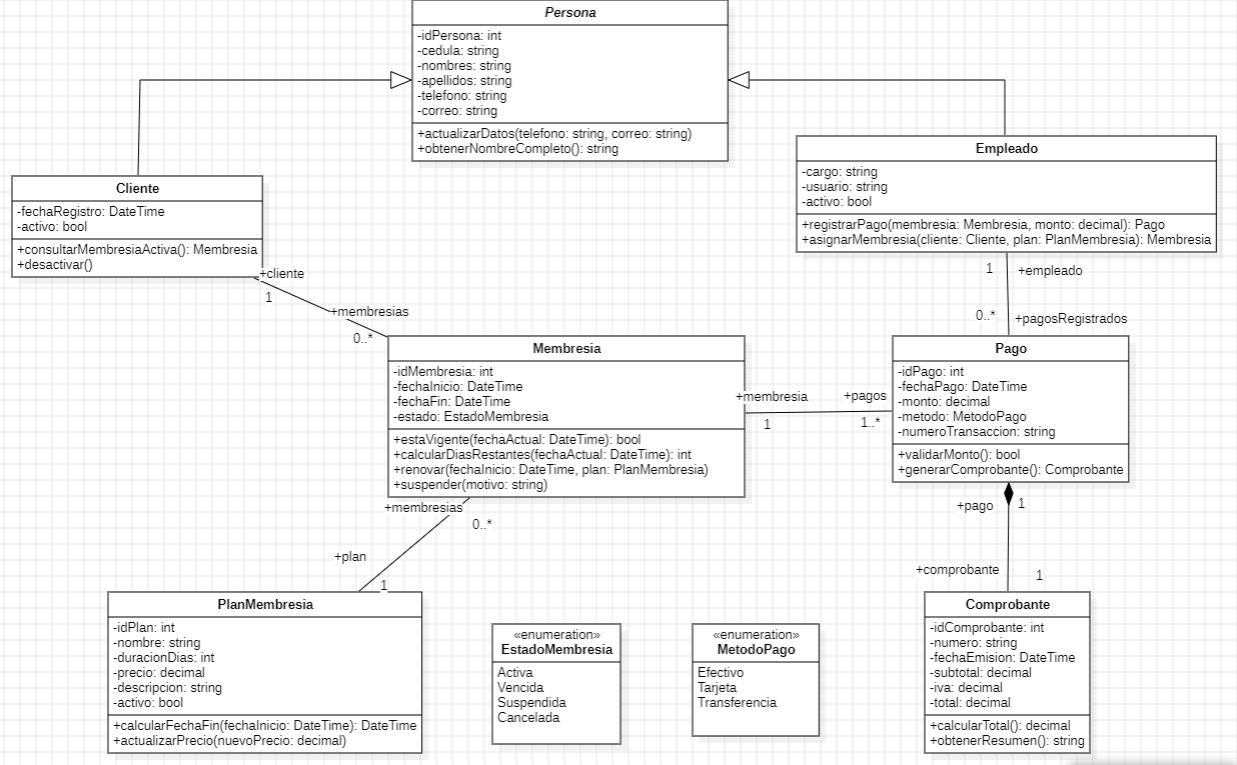
\includegraphics[width=\textwidth,height=0.52\textheight,keepaspectratio]
    {06_diagrama_clases_final.png}
  }{
    \fbox{\parbox[c][4.2cm][c]{0.90\textwidth}{\centering
      \textbf{Diagrama pendiente de insertar}\\[0.2cm]
      \texttt{diagrama\_clases\_subsistema.png}}}
  }
  \caption{Diagrama de clases del subsistema modelado}
  \label{fig:diagrama-clases-subsistema}
\end{figure}

\subsection{Clases del dominio}

\begin{sloppypar}
El modelo contiene siete clases: \texttt{Persona}, \texttt{Cliente},
\texttt{Empleado}, \texttt{PlanMembresia}, \texttt{Membresia}, \texttt{Pago}
y \texttt{Comprobante}. Además, emplea \texttt{EstadoMembresia} y
\texttt{MetodoPago} para restringir estados y métodos de pago. \texttt{Persona}
es abstracta y concentra los datos comunes de \texttt{Cliente} y
\texttt{Empleado}. Las responsabilidades detalladas se conservan en el
Anexo A.
\end{sloppypar}

\subsection{Atributos y operaciones}

Las clases incluyen identificadores y datos propios del dominio, junto con
operaciones de actualización, renovación, cálculo, validación y suspensión.
Todos los atributos tienen tipo y visibilidad, y las operaciones registran
parámetros y retorno. La tabla ampliada se presenta en el Anexo A para evitar
duplicar el contenido visible en el diagrama.

\subsection{Relaciones y cardinalidades}

Un cliente puede tener varias membresías; cada membresía corresponde a un plan
y contiene uno o varios pagos; un empleado puede registrar múltiples pagos;
y cada pago se compone con un comprobante. \texttt{Cliente} y
\texttt{Empleado} heredan de \texttt{Persona}. Las multiplicidades visibles
en el diagrama se trasladaron a referencias o colecciones tipadas.

\subsection{Estereotipos y perfiles utilizados}

El modelo utiliza elementos estándar de UML compatibles con la extensión de
C\# \cite{starumlCSharp2025}. No se añadieron perfiles ni estereotipos
específicos porque el generador trabajó directamente con clases,
enumeraciones, generalizaciones, asociaciones y composiciones.

\subsection{Validación sintáctica y semántica del modelo}

La revisión comprobó nombres, tipos, visibilidad, firmas, roles y
cardinalidades. StarUML 7.1.0 produjo el mensaje
\textit{VALIDATION RESULTS --- NO ERRORS}, por lo que el modelo quedó
validado con cero errores el 18 de julio de 2026.

\begin{figure}[htbp]
  \centering
  
\includegraphics[width=0.92\textwidth]{07_validacion_modelo_sin_errores.png}
  \caption{Validación del modelo en StarUML sin errores}
  \label{fig:validacion-modelo}
\end{figure}

\subsection{Archivo nativo del modelo en el repositorio}

El archivo nativo se almacenó como
\path{modelo/modelo_subsistema_gimnasio_corregido.mdj}. Su presencia en la
carpeta \path{modelo/} del repositorio debe verificarse nuevamente antes de la
entrega, porque el archivo \texttt{.mdj} es la evidencia reproducible del
modelo y no puede sustituirse únicamente por la imagen exportada.


\section{Configuración del generador}

\subsection{Generador o extensión utilizada}

Se utilizó \textit{C\# Extension for StarUML}, que interpreta el modelo
\texttt{.mdj} y genera archivos \texttt{.cs}. La ejecución se realizó sobre
el paquete base del subsistema y no sobre elementos aislados.

\subsection{Origen y versión del generador}

La extensión corresponde al paquete \texttt{staruml.csharp}, versión 0.9.7,
publicado por Dongjoon Lee con licencia MIT y compatibilidad declarada con
StarUML 6 o superior \cite{starumlCSharp2025}. Se ejecutó en StarUML 7.1.0.
Durante la verificación se detectaron tres valores de retorno inválidos para
C\#: \texttt{False}, \texttt{return null} en métodos \texttt{void} y
\texttt{return null} para \texttt{DateTime}. Se corrigió localmente la plantilla
\texttt{code-generator.js}; la copia modificada debe conservarse en
\path{plantillas/} junto con una nota que identifique el cambio.

\subsection{Lenguaje y plataforma objetivo}

El lenguaje objetivo es C\# y la plataforma de comprobación será .NET sobre
Windows. El código generado representará el dominio y posteriormente podrá
integrarse con Windows Forms, SQL Server Express y Dapper.

\subsection{Parámetros de generación}

\begin{table}[htbp]
  \centering
  \caption{Configuración resumida del generador}
  \label{tab:configuracion-generador}
  \footnotesize
  \begin{tabularx}{\textwidth}{>{\bfseries}p{4cm}X}
    \toprule
    Parámetro & Valor \\
    \midrule
    Paquete base & \texttt{Gimnasio.Dominio} \\
    Espacio de nombres & \texttt{Gimnasio.Dominio} \\
    Lenguaje & C\# \\
    Directorio de salida & \texttt{generado/src/Gimnasio.Dominio/} \\
    Convención & PascalCase para tipos; camelCase para miembros privados. \\
    Sobrescritura & Permitida solo en el directorio generado. \\
    \bottomrule
  \end{tabularx}
\end{table}

\subsection{Directorio de salida y convenciones de nombres}

Cada clase y enumeración se almacenará en un archivo del mismo nombre. Los
archivos manuales de prueba se ubicarán en
\texttt{generado/verificacion/}, fuera del directorio reemplazable.

\subsection{Política ante la regeneración}

Antes de regenerar se guardó el modelo y se separaron las carpetas
\path{Roundtrip/Antes/} y \path{Roundtrip/Despues/}. El directorio generado se
consideró reemplazable y no recibió lógica manual. Esta política permitió
comparar el resultado anterior y posterior sin confundirlo con
\texttt{Program.cs}.

\subsection{Decisiones de mapeo UML a código}

Los paquetes se mapearán a espacios de nombres; clases y enumeraciones a tipos
C\#; atributos a campos; operaciones a métodos; generalizaciones a herencia;
y multiplicidades múltiples a colecciones. La tabla ampliada de
correspondencia se encuentra en el Anexo A.

\subsection{Archivos de configuración en el repositorio}

La carpeta \path{plantillas/} conservará
\path{configuracion_generador.md}, \path{mapeo_uml_csharp.md} y los
archivos oficiales de la extensión necesarios para identificar su origen y
versión. Esto permitirá repetir el proceso sin depender únicamente de las
capturas.


\section{Proceso de generación}

\subsection{Preparación del entorno}

La prueba se realizó en Windows 11 de 64 bits con StarUML, la extensión C\#,
Visual Studio y el SDK de .NET instalados.

\begin{table}[htbp]
  \centering
  \caption{Entorno utilizado para la generación}
  \label{tab:entorno-generacion}
  \footnotesize
  \begin{tabularx}{0.88\textwidth}{>{\bfseries}p{4.2cm}X}
    \toprule
    Componente & Versión comprobada \\
    \midrule
    Sistema operativo & Windows 11, 64 bits \\
    StarUML & 7.1.0 (modo de prueba) \\
    Extensión C\# & 0.9.7 \\
    Visual Studio & Community 2026, versión 18.8.0 \\
    SDK y plataforma & .NET SDK 10.0.302; \texttt{net10.0} \\
    \bottomrule
  \end{tabularx}
\end{table}

\begin{figure}[htbp]
  \centering
  \begin{minipage}[t]{0.48\textwidth}
    \centering
    
\includegraphics[width=\linewidth,height=3.3cm,keepaspectratio]{01_version_staruml.png}
    \scriptsize (a) StarUML 7.1.0
  \end{minipage}\hfill
  \begin{minipage}[t]{0.48\textwidth}
    \centering
    
\includegraphics[width=\linewidth,height=3.3cm,keepaspectratio]{02_extension_csharp.png}
    \scriptsize (b) Extensión C\# 0.9.7 instalada
  \end{minipage}
  \caption{Versiones de StarUML y de la extensión de generación}
  \label{fig:versiones-staruml-extension}
\end{figure}

\subsection{Apertura y selección del modelo de origen}

Se abrió el archivo \texttt{modelo\_subsistema\_gimnasio\_corregido.mdj}, se
comprobó el diagrama y se seleccionó el paquete \texttt{Gimnasio.Dominio}. El
modelo se guardó antes de invocar el generador.

\subsection{Ejecución del generador}

El procedimiento aplicado fue: \textbf{1)} abrir \texttt{Tools}; \textbf{2)}
elegir \texttt{C\# $>$ Generate Code...}; \textbf{3)} seleccionar el paquete
base; y \textbf{4)} indicar
\texttt{generado/src/Gimnasio.Dominio/} como salida
\cite{starumlCSharp2025}.

\subsection{Registro o log de salida}

La extensión no mostró un cronómetro ni produjo un archivo de log exportable.
Como registro verificable se conservó la lista de los nueve archivos, sus
tamaños y la misma marca temporal de escritura: 18 de julio de 2026 a las
14:57:10. No se atribuyó a StarUML el tiempo de compilación medido por Visual
Studio.

\subsection{Árbol del proyecto generado}

El árbol mostró nueve archivos dentro del paquete base: siete clases y dos
enumeraciones. \path{Program.cs} y el archivo de proyecto de la aplicación de
consola pertenecen a la verificación manual y no se contabilizaron como
generados.

\subsection{Artefactos producidos}

Los archivos producidos fueron los siete tipos del dominio descritos en la
Sección 4.3 y las enumeraciones \texttt{EstadoMembresia.cs} y
\texttt{MetodoPago.cs}. No se atribuyeron a StarUML formularios, repositorios,
base de datos ni archivos creados manualmente.

\subsection{Tiempo de generación}

StarUML no expuso el tiempo transcurrido de generación. Los nueve archivos
quedaron registrados a las 14:57:10 del 18 de julio de 2026. Visual Studio sí
registró una compilación incremental de 0,061 segundos y una recompilación
completa de 3,888 segundos; estos valores corresponden a compilación, no a la
generación UML--C\#.

\begin{figure}[htbp]
  \centering
  \begin{minipage}[t]{0.48\textwidth}
    \centering
    \IfFileExists{figuras/01_version_staruml.png}{
      
\includegraphics[width=\linewidth,height=3.1cm,keepaspectratio]
      {01_version_staruml.png}
    }{\fbox{\parbox[c][2.5cm][c]{0.9\linewidth}{\centering Entorno pendiente}}}
    \scriptsize (a) Entorno y versiones
  \end{minipage}\hfill
  \begin{minipage}[t]{0.48\textwidth}
    \centering
    \IfFileExists{figuras/08_seleccion_paquete_generador.png}{
      \includegraphics[width=\linewidth,height=3.1cm,keepaspectratio]
      {08_seleccion_paquete_generador.png}
    }{\fbox{\parbox[c][2.5cm][c]{0.9\linewidth}{\centering Invocación pendiente}}}
    \scriptsize (b) Invocación del generador
  \end{minipage}

  \vspace{0.2cm}
  \begin{minipage}[t]{0.48\textwidth}
    \centering
    \IfFileExists{figuras/12_registro_archivos_generados.png}{
      \includegraphics[width=\linewidth,height=3.1cm,keepaspectratio]
      {12_registro_archivos_generados.png}
    }{\fbox{\parbox[c][2.5cm][c]{0.9\linewidth}{\centering Log pendiente}}}
    \scriptsize (c) Registro de salida
  \end{minipage}\hfill
  \begin{minipage}[t]{0.48\textwidth}
    \centering
    \IfFileExists{figuras/11_directorio_salida_generacion.png}{
      
\includegraphics[width=\linewidth,height=3.1cm,keepaspectratio]
      {11_directorio_salida_generacion.png}
    }{\fbox{\parbox[c][2.5cm][c]{0.9\linewidth}{\centering Árbol pendiente}}}
    \scriptsize (d) Árbol generado
  \end{minipage}
  \caption{Evidencias principales del proceso de generación}
  \label{fig:evidencias-generacion}
\end{figure}


\section{Verificación del código generado}

La verificación comprobó la estructura, sintaxis, compilación, ejecución y
fidelidad del código obtenido después de corregir la plantilla local del
generador.

\subsection{Estructura del proyecto generado}

Se verificó la presencia de nueve archivos \texttt{.cs}: siete clases y dos
enumeraciones, almacenados en \texttt{generado/src/Gimnasio.Dominio/}. Los
archivos manuales permanecieron en \texttt{generado/verificacion/}.

\subsection{Verificación sintáctica}

La revisión comprobó tipos, firmas, llaves, referencias y colecciones. La
primera generación reveló retornos inválidos introducidos por la extensión.
Después de corregir la plantilla y regenerar, la recompilación finalizó con
cero errores. Visual Studio mostró advertencias \texttt{CS0169} porque los
campos privados del esqueleto todavía no son utilizados; son coherentes con la
limitación de un generador estructural y no impidieron la ejecución.

\subsection{Compilación del código}

Como StarUML genera archivos fuente y no una solución ejecutable completa, se
usará un proyecto de consola manual que incluya las clases sin modificarlas.

\begin{lstlisting}[basicstyle=\ttfamily\footnotesize,frame=single,
caption={Comandos de verificación},label={lst:comandos-verificacion}]
cd generado/verificacion
dotnet restore
dotnet build
dotnet run
\end{lstlisting}

\textbf{Resultado:} .NET SDK 10.0.302, una recompilación correcta, cero
errores y advertencias \texttt{CS0169} por campos privados aún no utilizados.
La recompilación completa registrada duró 3,888 segundos.

\subsection{Ejecución de una unidad mínima demostrable}

El archivo manual \texttt{Program.cs} instanció los tipos generados y creó un
cliente, una membresía, un pago, un empleado y un comprobante. La consola
confirmó las relaciones con valores unitarios, mostró los retornos
predeterminados del esqueleto y finalizó con código de salida 0. Esta prueba
demuestra integración y ejecución en .NET, pero no constituye la
implementación completa de las reglas del gimnasio.

\begin{figure}[htbp]
  \centering
  \begin{minipage}[t]{0.48\textwidth}
    \centering
    \IfFileExists{figuras/17_compilacion_cero_errores.png}{
      \includegraphics[width=\linewidth,height=3.5cm,keepaspectratio]
      {17_compilacion_cero_errores.png}
    }{\fbox{\parbox[c][2.8cm][c]{0.9\linewidth}{\centering Compilación pendiente}}}
    \scriptsize (a) Resultado de \texttt{dotnet build}
  \end{minipage}\hfill
  \begin{minipage}[t]{0.48\textwidth}
    \centering
    \IfFileExists{figuras/18_ejecucion_codigo.png}{
      \includegraphics[width=\linewidth,height=3.5cm,keepaspectratio]
      {18_ejecucion_codigo.png}
    }{\fbox{\parbox[c][2.8cm][c]{0.9\linewidth}{\centering Ejecución pendiente}}}
    \scriptsize (b) Resultado de \texttt{dotnet run}
  \end{minipage}
  \caption{Compilación y ejecución del código generado}
  \label{fig:compilacion-ejecucion}
\end{figure}

\subsection{Correspondencia entre modelo y código}

\begin{table}[htbp]
  \centering
  \caption{Correspondencia representativa modelo--código}
  \label{tab:correspondencia-modelo-codigo}
  \scriptsize
  \begin{tabularx}{\textwidth}{>{\raggedright\arraybackslash}p{3.1cm}
    >{\raggedright\arraybackslash}p{3.4cm}X}
    \toprule
    Elemento UML & Código esperado & Resultado real \\
    \midrule
    \texttt{Persona} abstracta & Clase base abstracta. & \texttt{public abstract class Persona} \\
    Generalización de \texttt{Cliente} & Herencia de \texttt{Persona}. & \texttt{public class Cliente : Persona} \\
    \texttt{Membresia.estado} & Campo de tipo enumerado. & \texttt{private EstadoMembresia estado;} \\
    Cliente--Membresía \texttt{0..*} & Colección tipada. & \texttt{HashSet<Membresia> membresias;} \\
    Operación de suspensión & Método público con parámetro \texttt{string}. & \texttt{public void}\newline\texttt{suspender(string motivo)} \\
    \texttt{EstadoMembresia} & Archivo y declaración \texttt{enum}. & \texttt{EstadoMembresia.cs} \\
    \bottomrule
  \end{tabularx}
\end{table}

La correspondencia completa de clases, atributos, operaciones y relaciones se
traslada al Anexo A.

\subsection{Diferenciación entre código generado y código manual}

Los nueve archivos de \texttt{generado/src/} fueron producidos por StarUML.
\texttt{Program.cs}, el proyecto \texttt{.csproj} y los comandos de
verificación fueron manuales y permanecieron separados. La plantilla local
del generador sí fue corregida antes de regenerar; esto se documenta como una
configuración técnica del proceso, no como edición individual de los nueve
archivos resultantes.

\subsection{Limitaciones del generador}

La extensión genera principalmente estructura y presenta estas limitaciones:
\begin{itemize}[nosep]
  \item no implementa reglas de negocio ni cuerpos funcionales completos;
  \item no produce Windows Forms, Dapper, SQL Server ni la solución final;
  \item las asociaciones y colecciones deben revisarse después de generar;
  \item los cambios manuales dentro de la salida pueden perderse al regenerar.
\end{itemize}

Estas limitaciones no invalidan la prueba: delimitan qué automatiza StarUML y
qué deberá completarse manualmente en el PFC.


\section{Cierre del ciclo y roundtrip controlado}

\subsection{Estado inicial del modelo y del código}

El estado inicial se conservó en \path{Roundtrip/Antes/}. En
\texttt{Membresia.cs} aparecía la operación \texttt{renovar(...)} y la clase
finalizaba sin una operación de suspensión. El enlace al commit inicial queda
pendiente hasta que Erick publique esta evidencia en GitHub.

\subsection{Cambio realizado en el modelo UML}

Se añadió en StarUML la operación
\texttt{+suspender(motivo:string):void} a la clase \texttt{Membresia}. El
cambio se realizó en el modelo, sin editar previamente el archivo C\# de
salida.

\subsection{Regeneración del código}

Después de guardar el \texttt{.mdj}, se ejecutó nuevamente el mismo generador
sobre el paquete base. La nueva salida se almacenó en
\path{Roundtrip/Despues/}.

\subsection{Evidencia antes y después}

La evidencia compara \texttt{Membresia.cs} antes y después de la
regeneración. El estado posterior muestra la firma nueva y la recompilación
correcta.

\begin{figure}[htbp]
  \centering
  \begin{minipage}[t]{0.48\textwidth}
    \centering
    \includegraphics[width=\linewidth,height=4.0cm,keepaspectratio]{19_codigo_antes_roundtrip.png}
    \scriptsize (a) Antes: la clase termina después de \texttt{renovar}
  \end{minipage}\hfill
  \begin{minipage}[t]{0.48\textwidth}
    \centering
    \includegraphics[width=\linewidth,height=4.0cm,keepaspectratio]{20_codigo_despues_roundtrip.png}
    \scriptsize (b) Después: aparece \texttt{suspender(string motivo)}
  \end{minipage}
  \caption{Evidencia del roundtrip controlado en \texttt{Membresia.cs}}
  \label{fig:roundtrip-antes-despues}
\end{figure}

\subsection{Trazabilidad modelo a código}

La prueba fue satisfactoria: \texttt{Membresia.cs} incorporó
\texttt{public void suspender(string motivo)} y el proyecto volvió a compilar
con cero errores. La correspondencia conserva nombre, visibilidad, parámetro y
tipo de retorno definidos en UML.

\subsection{Manejo del código manual ante la regeneración}

El proyecto manual de verificación permanecerá fuera del directorio
sobrescrito. Después de regenerar se repetirá \texttt{dotnet build} para
confirmar que el cambio no afectó su compilación.


\section{Reparto del trabajo}

\subsection{Roles y responsabilidades}

La distribución prevista contempla cuatro responsabilidades diferenciadas:
modelado UML, configuración y generación, verificación técnica, y
documentación y presentación. Al cierre de este informe solo se confirmó el
aporte técnico de Erick; los roles de los demás integrantes permanecen
pendientes de confirmación y deben actualizarse antes de entregar.

\subsection{Tareas realizadas por integrante}

Erick realizó la configuración de StarUML, la corrección de la plantilla del
generador, la generación, la verificación en Visual Studio y el roundtrip. Los
demás integrantes deberán registrar tareas concretas y verificables, evitando
descripciones generales como ``ayudó en todo''.

\subsection{Commits atribuibles a cada integrante}

Todavía faltan commits sustantivos identificables de Steven, María y Jhon.
También debe publicarse el aporte técnico de Erick mediante su cuenta. Esta
sección no se completó con datos inventados porque la rúbrica exige autoría,
fecha y enlace verificables.

\subsection{Log de aportaciones de GitHub}

El historial completo se conservará en el Anexo E. Los commits deberán usar la
cuenta personal de cada integrante para que la autoría sea identificable.

\begin{figure}[htbp]
  \centering
  \includegraphics[width=0.88\textwidth]{23_estructura_repositorio_github.png}
  \caption{Estructura actual del repositorio público en GitHub}
  \label{fig:estructura-repositorio}
\end{figure}

\subsection{Participación en la exposición y demostración}

Los cuatro integrantes explicarán una parte diferenciada y participarán en la
demostración: teoría y justificación; modelo; generación y roundtrip; y
verificación, resultados y conclusiones.


\section{Conclusiones}

\subsection{Valor de MDD para el Proyecto Fin de Curso}

MDD permitió establecer una relación verificable entre el modelo del
subsistema y la estructura inicial del código. Las siete clases y dos
enumeraciones produjeron nueve archivos C\#, y el roundtrip demostró que una
operación añadida al modelo apareció en el archivo esperado. En el PFC este
proceso reduce tareas repetitivas si el modelo y la regeneración se controlan.

\subsection{Aprendizajes del equipo}

La actividad permitió diferenciar un diagrama usado solo como documentación
de un modelo que actúa como entrada de un generador. También evidenció la
necesidad de registrar versiones, parámetros, plantillas modificadas,
resultados y commits para que otra persona pueda repetir el proceso.

\subsection{Limitaciones identificadas}

StarUML generó principalmente la estructura del dominio y no reemplazó el
desarrollo de interfaces, persistencia ni reglas de negocio. La extensión
0.9.7 requirió una corrección local para emitir valores de retorno válidos en
C\#. El proyecto recompiló con cero errores, aunque mantuvo advertencias por
campos del esqueleto aún no utilizados. Estas limitaciones deben mostrarse en
la exposición como parte del resultado real.


\renewcommand{\refname}{Referencias bibliográficas}
\bibliographystyle{ieeetr}
\bibliography{referencias}
% ============================================================================
% ANEXOS (NO CUENTAN DENTRO DEL MAXIMO DE 20 PAGINAS)
% ============================================================================
\clearpage
\appendix

\section{Tabla ampliada de correspondencia modelo--código}
\label{anexo:correspondencia}

Este anexo conserva el detalle retirado del cuerpo para cumplir el límite de
páginas sin perder la definición técnica del modelo.

\footnotesize
\begin{longtable}{>{\raggedright\arraybackslash}p{3.1cm}
                  >{\raggedright\arraybackslash}p{5cm}
                  >{\raggedright\arraybackslash}p{6cm}}
\caption{Atributos y operaciones principales del dominio}\\
\toprule
\textbf{Clase} & \textbf{Atributos} & \textbf{Operaciones} \\
\midrule
\endfirsthead
\toprule
\textbf{Clase} & \textbf{Atributos} & \textbf{Operaciones} \\
\midrule
\endhead
\texttt{Persona} & idPersona, cedula, nombres, apellidos, telefono, correo & actualizarDatos(), obtenerNombreCompleto() \\
\texttt{Cliente} & fechaRegistro, activo, membresias & consultarMembresiaActiva(), desactivar() \\
\texttt{Empleado} & cargo, usuario, activo, pagosRegistrados & registrarPago(), asignarMembresia() \\
\texttt{PlanMembresia} & idPlan, nombre, duracionDias, precio, descripcion, activo & calcularFechaFin(), actualizarPrecio() \\
\texttt{Membresia} & idMembresia, fechaInicio, fechaFin, estado, cliente, plan, pagos & estaVigente(), calcularDiasRestantes(), renovar(), suspender() \\
\texttt{Pago} & idPago, fechaPago, monto, metodo, numeroTransaccion & validarMonto(), generarComprobante() \\
\texttt{Comprobante} & idComprobante, numero, fechaEmision, subtotal, iva, total & calcularTotal(), obtenerResumen() \\
\bottomrule
\end{longtable}
\normalsize

\begin{table}[htbp]
  \centering
  \caption{Reglas de mapeo UML a C\#}
  \footnotesize
  \begin{tabularx}{\textwidth}{>{\bfseries}p{3.5cm}XX}
    \toprule
    Elemento UML & Resultado C\# & Criterio de comprobación \\
    \midrule
    Paquete & Espacio de nombres y carpeta. & Coincidencia del nombre base. \\
    Clase & Clase y archivo \texttt{.cs}. & Una declaración por clase. \\
    Atributo & Campo con tipo y visibilidad. & Equivalencia de nombre y tipo. \\
    Operación & Método con parámetros y retorno. & Firma completa. \\
    Enumeración & Tipo \texttt{enum}. & Valores del modelo conservados. \\
    Multiplicidad múltiple & Colección tipada. & Tipo y cardinalidad revisados. \\
    Generalización & Herencia mediante dos puntos. & Clase base correcta. \\
    \bottomrule
  \end{tabularx}
\end{table}

\section{Fragmentos representativos del código generado}

Los siguientes fragmentos corresponden a estructuras producidas por StarUML
después de corregir la plantilla local. \texttt{Program.cs} no forma parte de
estos listados.

\begin{lstlisting}[style=codigoCSharp,caption={Herencia y colección generadas en Cliente.cs}]
public class Cliente : Persona {
    private DateTime fechaRegistro;
    private bool activo;
    public HashSet<Membresia> membresias;
}
\end{lstlisting}

\begin{lstlisting}[style=codigoCSharp,caption={Operación añadida mediante roundtrip en Membresia.cs}]
public void suspender(string motivo) {
    // TODO implement here
}
\end{lstlisting}

\begin{lstlisting}[style=codigoCSharp,caption={Enumeración generada en EstadoMembresia.cs}]
public enum EstadoMembresia {
    Activa, Vencida, Suspendida, Cancelada
}
\end{lstlisting}

\section{Evidencias complementarias}

Este anexo reunirá las capturas individuales del entorno, invocación, log,
árbol, compilación, ejecución y roundtrip, además de los archivos de registro.
En el cuerpo se mantendrán las composiciones necesarias para la evaluación.

\section{Instrucciones detalladas de reproducción}

\begin{enumerate}[nosep]
  \item clonar el repositorio y abrir el modelo \texttt{.mdj};
  \item comprobar las versiones de StarUML y de la extensión C\#;
  \item ejecutar el generador con los parámetros documentados;
  \item abrir \texttt{generado/verificacion/};
  \item ejecutar \texttt{dotnet restore}, \texttt{dotnet build} y \texttt{dotnet run};
  \item compilar el informe con PdfLaTeX, BibTeX y dos pasadas finales de
  PdfLaTeX.
\end{enumerate}

\section{Evidencia de contribuciones en GitHub}

\begin{table}[htbp]
  \centering
  \caption{Registro ampliado de contribuciones}
  \footnotesize
  \begin{tabularx}{\textwidth}{>{\raggedright\arraybackslash}p{3.5cm}X
    >{\raggedright\arraybackslash}p{2.5cm}
    >{\raggedright\arraybackslash}p{3cm}}
    \toprule
    Integrante & Aporte verificable & Fecha & Enlace al commit \\
    \midrule
    Díaz Pontón Steven Santiago & Aporte no reportado todavía & Pendiente & Pendiente \\
    Escudero Plaza María del Rosario & Aporte no reportado todavía & Pendiente & Pendiente \\
    Mera Arias Erick Jhair & Generación C\#, corrección de plantilla, verificación y roundtrip & 18-jul-2026 & Pendiente de publicar \\
    Mesías Quijije Jhon Alexander & Aporte no reportado todavía & Pendiente & Pendiente \\
    \bottomrule
  \end{tabularx}
\end{table}


\end{document}
